\documentclass[journal,a4paper]{IEEEtran}
\usepackage{graphicx}
\usepackage[spanish]{babel}
\usepackage[utf8]{inputenc}
\usepackage{hyperref}
\usepackage{xcolor,colortbl}
\usepackage{multirow}

% para hacer figuras
%\begin{figure}
%    \centering
%    \includegraphics[width=3.0in]{myfigure}
%    \caption{Simulation Results}
%    \label{simulationfigure}
%\end{figure}
\newcommand{\tit}[1]{\textsc{\textbf{#1}}}
\newcommand{\alto}{{\cellcolor{red!65} alto}}
\newcommand{\medio}{{\cellcolor{red!50!blue!65} medio}}
\newcommand{\bajo}{{\cellcolor{blue!65} bajo}}
\newcommand{\multi}[2]{\multirow{#1}{*}{\parbox{3.7cm}{#2}}}

\begin{document}

\title{Navegación autónoma para robots móviles usando visión estéreo}
\author{Cintia Corti, Carlos Augusto Lyon Di Pietro, Facundo Pessacg, Kevin Allekotte}

\maketitle

\begin{abstract}
Como trabajo final de la materia \textsc{Visión en robótica} de \textsc{DC.UBA.AR}
presentamos un método para la navegación autónoma de robots usando visión estéreo.
La implementación se realizó para el \textsc{Exabot} usando las librerías \textsc{OpenCV} y \textsc{LibElas}.
\end{abstract}

\section{Introducción}
En este trabajo presentamos un método para la navegación autónoma de un robot basado en algoritmos de computer vision usando cámaras en estereo.

\begin{figure}[h!]
    \centering
    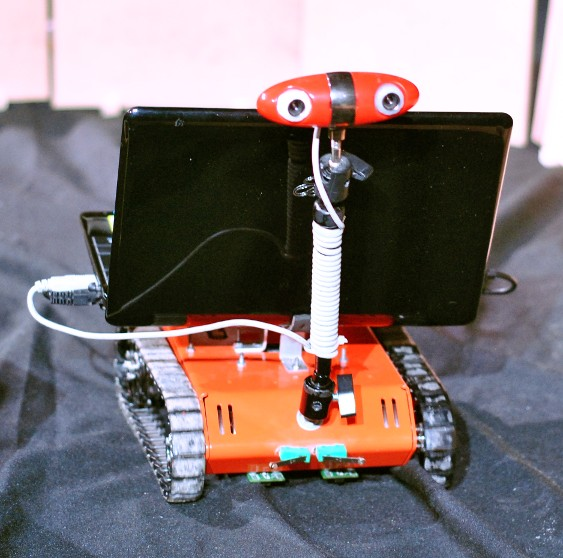
\includegraphics[width=0.9\linewidth]{exa.jpg}
    \caption{Exabot montado con cámara estereo y netbook.}
    \label{fig_exa}
\end{figure}

La visión en estéreo consiste de 2 cámaras alineadas en la misma dirección que toman las mismas imágenes desde puntos apartados ligeramente,
asemejandose al sistema de visión de los humanos y animales.
La idea es alinear las imagenes (previamente rectificadas) y calcular la disparidad en cada punto.
Cada punto del ambiente es captado por las 2 cámaras, y por propiedades trigonométricas vemos que la distancia del punto a las cámaras es proporcional a la diferencia de posicion horizontal observado entre las cámaras.
Así, un punto lejano va a proyectarse en las 2 imágenes en casi la misma posición, y un punto cercano a las cámaras va a proyectarse en posiciones distintas en cada cámara. 
Gracias a esta propiedad y calculando el mapa de disparidad entre las 2 imágenes podemos obtener una estimación muy buena de la geometría del espacio frente a las cámaras.
Un detalle no menor es que para calcular el mapa de disparidad de forma precisa las imágenes de las cámaras tienen que estar cuidadosamente rectificadas y alineadas. La rectificación corrige errores de deformación de las lentes para que las imágenes representen mas fielmente la proyección del espacio al plano de la cámara, y la alineación corrige la dirección en la que apuntan las cámaras para tener un sistema de referencia certero.

\begin{figure}[h!]
    \centering
    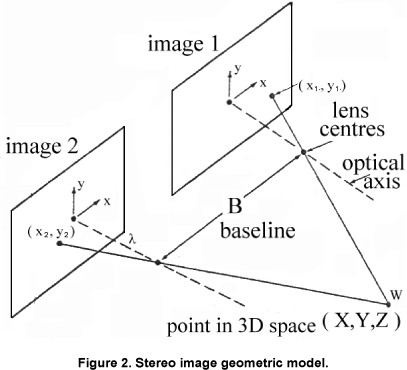
\includegraphics[width=0.9\linewidth]{stereo.jpg}
\end{figure}

El objetivo del método es permitir a un robot la navegación autónoma, por lo que es importante la performance para poder correr en tiempo real y proveer acciones correspondientes basado en la visión. Vamos a usar las librerías de \texttt{OpenCV} para procesar los streams de video y \texttt{LibElas} para calcular el mapa de disparidad.

Para llevar a cabo una navegación autónoma se debe implementar una estrategia basada en la observación del mundo (cámaras, mapa de disparidad) que decida acciones a ser llevadas a cabo por los actuadores (ruedas del exabot).
Buscamos una estrategia que evite la colisión con objetos y avance hacia espacios libres del ambiente.

\section{Método Propuesto}
\subsection{Calibración}
Las lentes de las cámaras tienen distorsiones que provocan que las imágenes captadas no representen exactamente la proyección de los objetos en el plano de captura. Por esto, y para obtener luego un mapa de disparidad preciso, es necesario aplicar las correcciones necesarias para ``rectificar'' las imágenes.

Para esto utilizamos software en el entorno \texttt{Matlab}, que permite calcular los parámetros intrínsecos y extrínsecos de las cámaras. Sacamos fotos estereoscopicas de una grilla -un damero- de dimensiones conocidas en distintas posiciones. Se indican características como origen y tamaño de la grilla, y el programa calcula las propiedades de la cámara como distancia focal, puntos principales, skew, dostorsión, rotación y distancia entre las cámaras.
Con estos parámetros podemos rectificar futuras capturas de la cámara para obtener imágenes alineadas y listas para procesar.

\begin{figure}[h!]
    \centering
    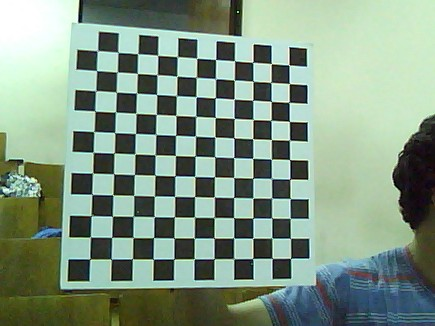
\includegraphics[width=0.8\linewidth]{calibracion1.jpg}
    
    \medskip
    
    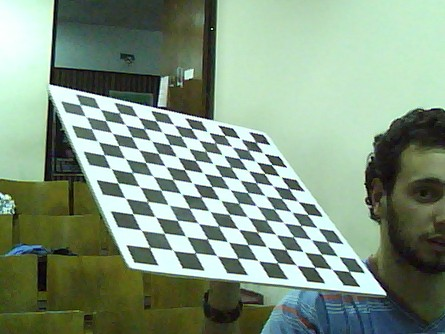
\includegraphics[width=0.8\linewidth]{calibracion2.jpg}
    \caption{Imagenes de prueba para calcular los parametros de rectificacion}
    \label{fig_calibracion}
\end{figure}

\subsection{Mapa de Disparidad}
Con las imágenes correctamente rectificadas podemos usarlas para calcular el mapa de disparidad.
Para esto vamos a usar la librería \texttt{LibElas} --Library for Efficient Large-scale Stereo Matching-- desarrollada por Andreas Geiger (Karlsruhe Institute of Technology).

\begin{figure}[h!]
    \centering
    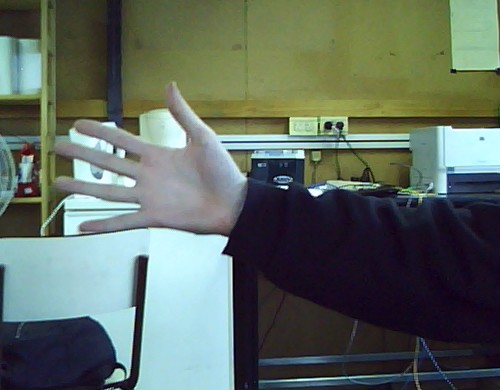
\includegraphics[width=0.9\linewidth]{libelas1.jpg}
    
    \medskip
    
    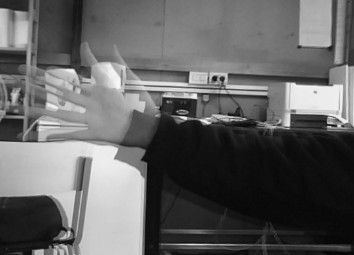
\includegraphics[width=0.9\linewidth]{libelas2.jpg}
    
    \medskip
    
    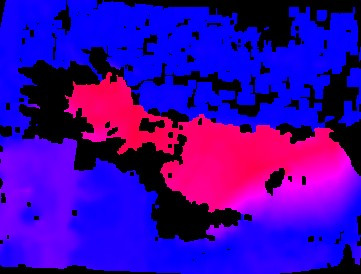
\includegraphics[width=0.9\linewidth]{libelas3.jpg}
    \caption{Una cámara; rectificadas y alineadas; mapa de disparidad}
    \label{fig_libelas}
\end{figure}

En la figura \ref{fig_libelas} podemos ver primero una imagen tal cual es captada por una de las cámaras, luego las 2 imágenes superpuestas (rectificadas y alineadas), y la tercera es el mapa de disparidad que obtenemos de la librería elas.

Este mapa de disparidad fue coloreado para entenderlo mejor visualmente, pero es simplemente un campo escalar donde la ``intensidad'' de un pixel representa la cercanía de un objeto en ese punto.
Observamos que hay zonas en negro, donde no tenemos información de la profundidad. Esto puede deberse a que no hay suficiente contraste en esas partes de la imagen, o que el algoritmo no encontró matches entre las 2. Hay que tener esto en cuenta a la hora de usar el mapa, pero igualmente es usable para nuestro propósito de navegación autónoma.

\subsection{Parametrización de atributos}
Para que el mapa de disparidad recién calculado sea útil, es necesario extraer información de éste que pueda usarse en la decisión de las acciones a tomar.

Dado que las acciones razonables que puede realizar un robot como el exabot para navegar ambientes son: avanzar, avanzar hacia la izquierda, avanzar hacia la derecha o girar en el lugar, vamos a analizar la presencia de obstáculos en alguna de estas direcciones.

Definimos 3 áreas disjuntas del campo de vision del robot --izquierda, centro y derecha-- y nuestro método se basa en decidir si hay espacio para avanzar en estas direcciones.
Descartamos un porcentaje (10\%) del borde de la imagen que consideramos que tiene ruido, especialmente luego de rectificar y alinear las imágenes, y la dividimos horizontalmente en 3 áreas iguales.
A cada una de estas áreas le calculamos el promedio de la intensidad de los pixels, llamamos \texttt{p\_izq}, \texttt{p\_med} y \texttt{p\_der}.

Esto nos da una idea del espacio que hay frente al robot en estas regiones.
Si el promedio es relativamente alto, significa que hay puntos del ambiente que estan cerca de la cámara, y por lo tanto, que hay obstáculos en esa dirección.
Si por el contrario el promedio es un valor bajo, podemos asumir que hay espacio libre para avanzar.
Definimos arbitrariamente 2 umbrales para los valores de los promedios. Si un valor supera el umbral alto consideramos que hay un obstáculo muy cercano y que no es seguro avanzar en esa dirección; si está entre los 2 umbrales hay algo frente al robot pero no es crítico; y si esta por debajo del umbral bajo consideramos que el camino está libre.

Además, para tener estimaciones más precisas de los valores reales, promediamos cada valor también en el tiempo. Es decir, calculamos \texttt{p\_izq}, \texttt{p\_med} y \texttt{p\_der} para cada frame durante un tiempo determinado, y luego promediamos el valor de cada área.

\begin{figure}[h!]
    \centering
    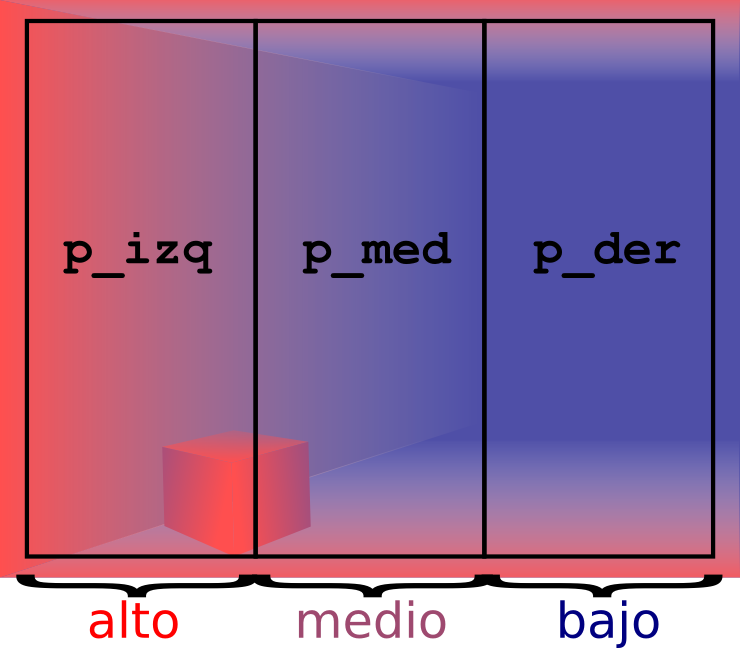
\includegraphics[width=0.9\linewidth]{disparidad.png}
    \caption{Análisis del mapa de disparidad}
    \label{fig_disparidad}
\end{figure}

En resumen, cada cierta cantidad de frames obtenemos estimaciones de la cercanía de obstáculos para cada una de las 3 áreas. Esto nos identifica 27 posibles escenarios para tomar decisiones en cada instante. Elegimos la cantidad de frames a promediar en función de los FPS para tomar una decisión cada aproximadamente 3 segundos.

\subsection{Estrategia}
Para llevar a cabo la navegación necesitamos una estrategia que determine qué acciones tomar ante cada escenario posible.
Usamos la categorización de posibilidades que mencionamos recién, y vamos a enumerar las acciones a tomar en cada caso.

En la siguiente tabla [\ref{tbl_estrategia}] se presenta la accion a tomar según los valores de los promedios de las áreas.
La estrategia está pensada para que explore lo máximo posible sincolisionar con abstáculos.

\begin{figure}[h!]
    \centering
    \begin{tabular}{|c|c|c|p{3.7cm}|}
    \hline
    \texttt{p\_izq} & \texttt{p\_med} & \texttt{p\_der} & \textbf{Acción} \\
    \hline
    \hline
    \bajo & \bajo & \bajo & \multi{4}{avanzar rápido}\\
    \cline{1-3}
    \bajo & \bajo & \medio & \\
    \cline{1-3}
    \medio & \bajo & \bajo & \\
    \cline{1-3}
    \medio & \bajo & \medio & \\

    \hline
    \bajo & \bajo & \alto & \multi{2}{avanzar hacia la izquierda}\\
    \cline{1-3}
    \medio & \bajo & \alto & \\

    \hline
    \alto & \bajo & \bajo & \multi{2}{avanzar hacia la derecha}\\
    \cline{1-3}
    \alto & \bajo & \medio & \\

    \hline
    \alto & \bajo & \alto & avanzar lento\\

    \hline
    \hline
    \bajo & \medio & \bajo & avanzar lento\\

    \hline
    \bajo & \medio & \medio & \multi{2}{avanzar lento hacia la izquierda}\\
    \cline{1-3}
    \bajo & \medio & \alto & \\

    \hline
    \medio & \medio & \bajo & \multi{2}{avanzar lento hacia la derecha}\\
    \cline{1-3}
    \alto & \medio & \bajo & \\

    \hline
    \alto & \medio & \alto & \multi{4}{avanzar muy lento}\\
    \cline{1-3}
    \medio & \medio & \medio & \\
    \cline{1-3}
    \alto & \medio & \medio & \\
    \cline{1-3}
    \medio & \medio & \alto & \\

    \hline
    \hline
    \bajo & \alto & \bajo & \multi{3}{girar}\\
    \cline{1-3}
    \medio & \alto & \medio & \\
    \cline{1-3}
    \alto & \alto & \alto & \\

    \hline
    \bajo & \alto & \medio & \multi{3}{girar a la izquierda}\\
    \cline{1-3}
    \bajo & \alto & \alto & \\
    \cline{1-3}
    \medio & \alto & \alto & \\

    \hline
    \medio & \alto & \bajo & \multi{3}{girar a la derecha}\\
    \cline{1-3}
    \alto & \alto & \bajo & \\
    \cline{1-3}
    \alto & \alto & \medio & \\
    \hline
    \end{tabular}
    
    \caption{Estrategia de navegación}
    \label{tbl_estrategia}
\end{figure}

Observar que la acción a tomar en cada caso es determinística y sólo depende del estado actual del sensado (o de los últimos ~3 segundos de sensado).

Por ejemplo, en el caso de la figura \ref{fig_disparidad} (donde los valores de los promedios son \emph{alto}, \emph{medio}, \emph{bajo}, la estrategia dice que hay que avanzar lento hacia la derecha.

Cada una de estas acciones se traduce a un par de velocidades para los motores que producen que el robot haga esa acción. En el ejemplo, ``avanzar lento hacia la derecha'' se traduce a (0.216, 0.072), osea una velocidad de 0.216 para el motor izquierdo y 0.072 para el derecho. El efecto producido es que el exabot avanza levemente mientras rota hacia la derecha.

\section{Experimentos}

\section{Conclusiones}

\section{Bibliografía}

\tit{LibElas}: Librería para computar mapas de disparidad a partir de pares de imagenes en escala de grises rectificadas. \url{http://www.cvlibs.net/software/libelas.html}

\bigskip

\tit{OpenCV}: Librería de funciones para computer vision en tiempo real. \url{http://opencv.willowgarage.com/}
\end{document}
